\documentclass{beamer}



\mode<presentation> {
%\mode<handouts> {
%\mode<article> {


% The Beamer class comes with a number of default slide themes
% which change the colors and layouts of slides. Below this is a list
% of all the themes, uncomment each in turn to see what they look like.


%\usetheme{default}
%\usetheme{AnnArbor}
%\usetheme{Antibes}
%\usetheme{Bergen}
%\usetheme{Berkeley}
%\usetheme{Berlin}
%\usetheme{Boadilla}
\usetheme{CambridgeUS}
%\usetheme{Copenhagen}
%\usetheme{Darmstadt}
%\usetheme{Dresden}
%\usetheme{Frankfurt}
%\usetheme{Goettingen}
%\usetheme{Hannover}
%\usetheme{Ilmenau}
%\usetheme{JuanLesPins}
%\usetheme{Luebeck}
%\usetheme{Madrid}
%\usetheme{Malmoe}
%\usetheme{Marburg}
%\usetheme{Montpellier}
%\usetheme{PaloAlto}
%\usetheme{Pittsburgh}
%\usetheme{Rochester}
%\usetheme{Singapore}
%\usetheme{Szeged}
%\usetheme{Warsaw}

% As well as themes, the Beamer class has a number of color themes
% for any slide theme. Uncomment each of these in turn to see how it
% changes the colors of your current slide theme.

%\usecolortheme{albatross}
\usecolortheme{beaver}
%\usecolortheme{beetle}
%\usecolortheme{crane}
%\usecolortheme{dolphin}
%\usecolortheme{dove}
%\usecolortheme{fly}
%\usecolortheme{lily}
%\usecolortheme{orchid}
%\usecolortheme{rose}
%\usecolortheme{seagull}
%\usecolortheme{seahorse}
%\usecolortheme{whale}
%\usecolortheme{wolverine}

%\setbeamertemplate{footline} % To remove the footer line in all slides uncomment this line
%\setbeamertemplate{footline}[page number] % To replace the footer line in all slides with a simple slide count uncomment this line

%\setbeamertemplate{navigation symbols}{} % To remove the navigation symbols from the bottom of all slides uncomment this line
}

\usepackage{graphicx} % Allows including images
\graphicspath{{../figures}}
\usepackage{booktabs} % Allows the use of \toprule, \midrule and \bottomrule in tables
\usepackage{amsmath, amssymb, amsthm, gensymb,mathrsfs}%,eufrak}
\usepackage{hyperref}
\usepackage{tabularx}
\usepackage{longtable}
\usepackage{makecell}
\usepackage{multicol}
\usepackage{physics}
\usepackage{tikz}

\newcommand{\uvec}[1]{\ensuremath{\textbf{#1}}}
%\newcommand{\r1}{\ensuremath{\mathbb{R}}}
\newcommand{\rn}[1]{\ensuremath{\mathbb{R}^{#1}}}

\newcounter{excounter}
%\renewcommand{\thefpcounter}{\thechapter.\arabic{fpcounter}}
%\renewcommand{\thefpcounter}{\thesection.\arabic{fpcounter}}
\renewcommand{\theexcounter}{\arabic{excounter}}

%\newtheorem{exercici}{Exercici}
% \newenvironment{exercici}[1]{%
% \refstepcounter{excounter}%
% \label{#1}%
% \noindent\textbf{Exercixi~\theexcounter}%
% \setbeamercolor{block title example}{fg=blue,bg=red!75!black}%
% \begin{example}#2[#1]}{\end{example}
% \vspace{\baselineskip}
% }%
% {}%

\newenvironment{exercici}[1]{%
\refstepcounter{excounter}%
\label{#1}%
\noindent\textbf{Exercici~\theexcounter}%
}%
{}%

\newtheorem{teorema}{Teorema}[section]
\newtheorem{definicio}{Definició}[section]

\usepackage[T1]{fontenc}
%\usepackage[utf8]{inputenc}
\usepackage[catalan]{babel}
%\usepackage{lmodern}


\usepackage{fancyvrb}
\usepackage{xcolor}
\usepackage{listings}
\lstset{language=python,
    basicstyle=\ttfamily,
    commentstyle=\color{red},
    keywordstyle=\color{blue},
    captionpos=b,
    backgroundcolor=\color{lightgray},
    showstringspaces=false
}

\renewcommand{\lstlistingname}{Code}

\definecolor{links}{HTML}{2A1B81}
\hypersetup{colorlinks,linkcolor=,urlcolor=links}
\setbeamertemplate{caption}[numbered]%   

%----------------------------------------------------------------------------------------
%	 TITLE PAGE
%----------------------------------------------------------------------------------------

\title[Àlgebra]{Vectors i Valors propis} % The short title appears at the bottom of every slide, the full title is only on the title page
\author{Jordi Villà i Freixa} % Your name
\institute[FCTE] % Your institution as it will appear on the bottom of every slide, may be shorthand to save space
{
Universitat de Vic - Universitat Central de Catalunya \\
Grau en Enginyeria Mecatrònica\\ % Your institution for the title page
\medskip
\textit{jordi.villa@uvic.cat} % Your email address
}
%\date{\today} % Date, can be changed to a custom date
\date{curs 2023-2024}
\logo{
\includegraphics[width=.1\textwidth]{FCTE}}
\begin{document}

\begin{frame}
\titlepage % Print the title page as the first slide
\end{frame}

\begin{frame}
\frametitle{Índex} % Table of contents slide, comment this block out to remove it
\tableofcontents % Throughout your presentation, if you choose to use \section{} and \subsection{} commands, these will automatically be printed on this slide as an overview of your presentation
\end{frame}

\begin{frame}
    \frametitle{Referències}
    El material d'aquestes presentacions està basat en anteriors presentacions i apunts d'altres professors \cite{jlgarcia,mcorbera,mcalle} de la UVic-UCC, pàgines web diverses (normalment enllaçades des del text), així com monografies.
\end{frame}

\section{Valors i vectors propis}

\begin{frame}
  \frametitle{Valors i vectors propis}

  \begin{definicio}
    Sigui $A\in \mathcal{M}_n (\mathbb{C})$; és a dir, unja matriu quadrada amb elements complexos. Direm que $\lambda\in \mathbb{C}$ és un {\bf valor propi (vap)}  d'$A$ si existeix algun vector no nul $\uvec{u}\in \mathbb{C}$ tal que $A\uvec{u}=\lambda\uvec{u}$. Aquest vector $\uvec{u}$ s'anomena {\bf vector propi (vep) associat al valor propi $\lambda$.}
  \end{definicio}

  \begin{exercici}{}
    Demostra que els valors propis d'$A=\begin{pmatrix}2&-2\\0&3\end{pmatrix}$ són $\alpha_1=2$ i $\alpha_2=3$ i troba els corresponents vectors propis.
  \end{exercici}
\end{frame}


\begin{frame}
  \frametitle{Càlcul de vectors i valors propis}
  El que acabem de descriure ens mostra també com calcular els vectors i valors propis. Si $I$ és la matriu identitat d'ordre $n$:
  \begin{enumerate}
    \item $A\uvec{u}-\alpha \uvec{u}=\uvec{0}$
    \item $(A-\alpha I)\uvec{u}=\uvec{0}$
    \item $\det(A-\alpha I)=0$, que genera l'anomenat {\bf polinomi característic} de la matriu $A$.
  \end{enumerate}
  I deduïm també que el vector $\uvec{v}$ pertany al nucli de l'aplicació $(A-\alpha I)$. Els valors propis seran les arrels del polinomi característic i per trobar el vector propi associat a cada arrel caldrà resoldre els sistemes $A\uvec{u}=\alpha \uvec{u}$ o, equivalentment, $(A-\alpha I)\uvec{u}=\uvec{0}$.

  \begin{exercici}{}
    Trobar els valors i vectors propis de les matris $A=\begin{pmatrix}1&1\\3&-1\end{pmatrix}$ i $B=\begin{pmatrix}2&1&-1\\1&2&0\\-1&1&2\end{pmatrix}$
  \end{exercici}
\end{frame}
%------------------------------------------------
%------------------------------------------------
\section{Diagonalització}
%------------------------------------------------
%------------------------------------------------
\begin{frame}
  \frametitle{Matrius semblants i diagonalització}
  Dues matrius $A$ i $B$ són semblants si existeix una matriu $P$ no singular ($\det(P) \neq 0$) tal que $B=P^{-1}\cdot A \cdot P$.

  \begin{exercici}{}
    Comprova que les matrius
    $A=\begin{pmatrix}2&1&-1\\1&2&0\\-1&1&2\end{pmatrix}$ i
    $B=\begin{pmatrix}3&0&0\\0&\frac{3-\sqrt{5}}{2}&0\\0&0&\frac{3+\sqrt{5}}{2}\end{pmatrix}$
    són semblants amb
    $P=\begin{pmatrix}1&1&1\\1&\frac{1-\sqrt{5}}{2}&\frac{1+\sqrt{5}}{2}\\0&1&1\end{pmatrix}$
  \end{exercici}

  \vspace{\baselineskip}
  {\bf Les matrius semblants representen la mateixa aplicació lineal en dues bases diferents, essent $P$ la matriu de canvi de base.}

\end{frame}

%------------------------------------------------
%------------------------------------------------
\begin{frame}{Diagonalització}
  \begin{definicio}
    Direm que la matriu $A\in \mathcal{M}_n (\mathbb{C})$ és {\bf diagonalitzable} si existeix una matriu inversible $C\in \mathcal{M}_n (\mathbb{C})$ i una matriu diagonal $D\in \mathcal{M}_n (\mathbb{C})$ tal que $A=C\cdot D \cdot C^{-1}$ (o bé $D=C^{-1}\cdot A \cdot C$). La matriu $C$ s'anomena {\bf matriu de canvi de base}.
  \end{definicio}
\end{frame}
\begin{frame}
  \begin{teorema}
    Si $A\in \mathcal{M}_n (\mathbb{C})$ té $n$ valors propis diferents $\lambda_1,\lambda_2,\ldots, \lambda_n$, llavors $A$ diagonalitza; és a dir, existeix una matriu inversible $C$ i una matriu diagonal $D$ tal que $A=C\cdot D \cdot C^{-1}$. A més,
    \[
      D=\begin{pmatrix} 
        \lambda_1 & 0 & \cdots & 0\\
        0 & \lambda_2 & \cdots & 0\\
         &  & \ddots & \\ 
        0 & 0 & \cdots & \lambda_n
      \end{pmatrix}                      
    \]
    i la matriu $C$ està formada per $n$ vectors propis de valors propis respectius $\lambda_1,\lambda_2,\ldots, \lambda_n$ (en columnes).
  \end{teorema}
\end{frame}
%------------------------------------------------
%------------------------------------------------
\begin{frame}
  \begin{exercici}{Diagonalització}
    Diagonalitza la matriu $A=\begin{pmatrix}1&2\\2&1\end{pmatrix}$ i interpreta aquesta imatge en termes de l'efecte de la matriu sobre els seus vep.
  \begin{figure}
    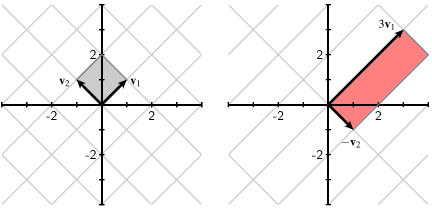
\includegraphics[scale=0.5]{eigen}
  \end{figure}
\end{exercici}
\end{frame}
%------------------------------------------------
%------------------------------------------------
\begin{frame}
  \begin{enumerate}
    \item Si $A$ i $B$ són semblants, tenen els mateixos valors propis
    \item Respecte els vectors propis:
    \begin{itemize}
      \item si $\uvec{v}$ és vector propi d'$A$, $\uvec{v'}=P^{-1}\uvec{v}$ ho és de $B$.
      \item si $\uvec{v'}$ és vector propi de $B$, $\uvec{v}=P\uvec{v'}$ ho és d'$A$.
    \end{itemize}
    \item $A$ és invertible (no singular) $\Leftrightarrow$ 0 no és un valor propi d'$A$.
    \item $\alpha \neq 0$ és un valor propi d'$A$ de vector propi $\uvec{v}\Rightarrow \frac{1}{\alpha}$ és un valor propi d'$A^{-1}$ de vector propi $\uvec{v}$
    \item si $\alpha_1,\alpha_2, \ldots, \alpha_n$ són valors propis d'$A$, $\Rightarrow \left\{ \begin{matrix}tr(A)=\alpha_1+\alpha_2+ \cdots + \alpha_n\\\det(A)=\alpha_1 \cdot \alpha_2 \cdots  \alpha_n\end{matrix}\right.$
    \item $A$ és diagonalitzable si és semblant a una matriu diagonal: $D=P^{-1}AP$.
    \item Tota matriu simètrica de coeficients reals és diagonalitzable i té valors propis reals.
  \end{enumerate}
\end{frame}
%------------------------------------------------
%------------------------------------------------
%------------------------------------------------
%------------------------------------------------
\begin{frame}

  \begin{exercici}{}
    Calcula $\begin{pmatrix}1&1\\3&-1\end{pmatrix}^6$
  \end{exercici}

  \begin{exercici}{}
    Estudia si aquestes matrius són diagonalitzables:
    $A=\begin{pmatrix}1&1&a\\0&-1&0\\a&1&1\end{pmatrix}$, $A=\begin{pmatrix}1&a&a\\-1&1&-1\\1&0&2\end{pmatrix}$,
    $A=\begin{pmatrix}0&1&1\\0&0&4\\0&0&3\end{pmatrix}$
  \end{exercici}

  \begin{exercici}{}
    Té valors propis reals una matriu de rotació?
  \end{exercici}

\end{frame}


\begin{frame}
    \frametitle{References}
    
    \footnotesize{
    \begin{thebibliography}{99} % Beamer does not support BibTeX so references must be inserted manually as below
    
    \begin{columns}[t]
      \column{.45\textwidth}
    
    \bibitem[VanVerth, 2015]{vanverth} James M. Van Verth, Lars M. Bishop (2015)
    \newblock Essential Mathematics for Games and Interactive Applications
    \newblock \emph{Elsevier}.
    
    \bibitem[Riley, 2002]{riley} K.F. Riley, M.P. Hobson, S.J. Bence (2002)
    \newblock Mathematical Methods for Physics and Engineering (2nd Ed)
    \newblock \emph{McGraw Hill}.
    
    \bibitem[Lipschutz, 2001]{schaum} Seymour Lipschutz, Marc Lipson (2001)
    \newblock Schaum's outlines: Linear Algebra (3rd Ed)
    \newblock \emph{McGraw Hill}.
    
    \column{.45\textwidth}
    
    \bibitem[García]{jlgarcia} Josep Lluís García
    \newblock Presentacions Matemàtiques Grau en Multimèdia, Aplicacions i Videojocs
    \newblock \emph{UVic-UCC}.
    
    \bibitem[Corbera]{mcorbera} Montserrat Corbera, Vladimir Zaiats
    \newblock Apunts d'Àlgebra Lineal
    \newblock \emph{UVic-UCC}.
    
    \bibitem[Calle]{mcalle} Malu Calle
    \newblock Apunts d'Àlgebra Lineal
    \newblock \emph{UVic-UCC}.
    
    \end{columns}
    \end{thebibliography}
    
    }
    \end{frame}

\end{document}
